%!TEX encoding = UTF-8 Unicode
%!TEX root = ../compendium.tex

\chapter{Terminalfönster}\label{appendix:terminal}

\section{Vad är ett terminalfönster?}

I ett terminalfönster kan man skriva kommandon som kör program och hanterar filer. När man programmerar använder man ofta terminalkommando för att kompilera och exekvera sina program.  
 
\subsubsection{Terminal i Linux}

    \begin{figure}[!b]
    \centering
    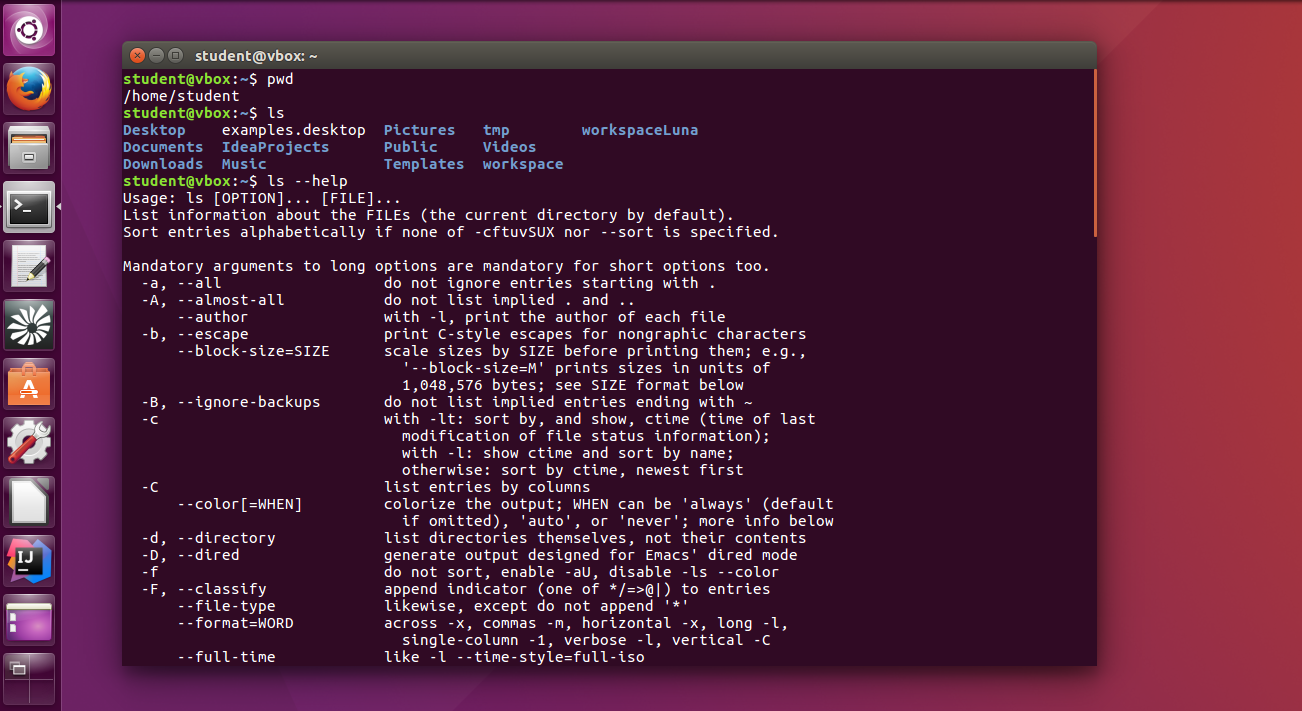
\includegraphics[width=1.0\textwidth]{../img/linux-terminal.png}
    \caption{Terminalfönster i Ubuntu öppnas med Ctrl+Alt+T.}
    \label{fig:terminal:linux}
    \end{figure}

I Linux används ofta kortkommando för att starta ett terminalfönster. I Ubuntu trycker man Ctrl+Alt+T.  Då öppnas ett fönster med en blinkande markör som visar att det är redo att ta emot dina textkommando. Ett exempel på kommando är \texttt{ls} som skriver ut en lista med filer i det aktuella biblioteket, så som visas i fig. \ref{fig:terminal:linux}.

Det som visas i ett terminalfönster sköts av ett \textbf{kommandoskal} \Eng{command shell}, som är redo att ta emot kommando efter en prompt som slutar med ett \texttt{\$}-tecken. När du skriver ett kommando och trycker Enter anropar kommandoskalet en kommandotolk som tolkar och utför dina kommandon. Om ett kommando inte kan tolkas, skrivs ett felmeddelande. Det finns många användbara kortkommando, varav de viktigaste visas i tabell \ref{fig:terminal:shortcuts}. Det är bra om du lär dig dessa kortkommandon utantill så att ditt arbete i terminalen går snabbt och smidigt.

\begin{table}[H]
\renewcommand{\arraystretch}{1.15}
\begin{tabular}{@{}r | l}
Ctrl+A & flytta markören till början av raden \\
Ctrl+E & flytta markören till slutet av raden \\
Tab & ''auto-complete'', fyll i resten baserat på vad du skrivit hittills \\
Tab Tab & två tryck på Tab listar eventuella alternativ \\
Ctrl+K & ''kill'', ta bort tecken från markören till radens slut\\
Ctrl+U & ta bort tecken från markören till början av raden \\
Ctrl+Y & ''yank'', sätt in det som senast togs bort\\
Ctrl+Z & stoppa pågående process, skriv sedan \texttt{bg} för bakgrundskörning\\
Ctrl+L & rensa terminalfönstret\\
Ctrl+D & avsluta kommandoskalet \\
\end{tabular}
    \caption{Viktiga kortkommandon i Linux terminalfönster.}
    \label{fig:terminal:shortcuts}
\end{table}

\noindent Ctrl+C orsakar normalt ett avbrott av pågående process, men om du vill att Ctrl+C ska vara ''Copy'' som vanligt för att kopiera markerad text, kan du ställa om detta med terminalförnstrets  meny ''Edit $\rightarrow$ Keyboard Shortcuts'', eller liknande.




 
\subsubsection{PowerShell och Cmd i Microsoft Windows}
Microsoft Windows är inte Linux-baserat, men i kommandotolken PowerShell finns alias definierade för några vanliga Linux-kommandon, inkluderat \texttt{ls}, \texttt{cd} och \texttt{pwd}. Du startar Powershell t.ex. genom att trycka på Windows-knappen och skriva \texttt{powershell}. Du kan också, medan du bläddrar bland filer, klicka på filnamnsraden överst i filbläddraren och skriva \texttt{powershell} och tryck Enter. Ändra gärna typsnitt och bakgrundsfärg med hjälp av fönstrets menyer, så att det blir lättare för dig att läsa vad som skrivs.

Det finns även i Windows den ursprungliga kommandotolken Cmd med helt andra kommandon. Till exempel skriver man i Cmd kommandot \texttt{dir} i stället för \texttt{ls} för att lista filer. 



\subsubsection{Terminal i Apple OS X / macOS}


Apple OS X och macOS är Unix-baserade operativsystem. De flesta vanliga terminalkommandon som fungerar i Linux fungerar också under Apple OS X och macOS. Fråga någon om hjälp om du inte hittar hur man öppnar terminalfönstret.



\section{Några viktiga terminalkommando}

I tabell \ref{fig:terminal:commands} nedan finns en lista med några viktiga terminalkommando som är bra att lära sig utantill.

\begin{table}[H]
\renewcommand{\arraystretch}{1.15}
   
\begin{tabular}{@{}r | l}
\texttt{ls} & lista filer i aktuellt bibliotek (alltså där du ''står'')\\
\texttt{ls -A} & lista alla filer i aktuellt bibliotek, även gömda \\
\texttt{man ls} & manual för kommandot \texttt{ls}; testa även för andra kommandon! \\
\texttt{cd} \textit{d} & ''change directory'', ändra aktuellt bibliotek till \textit{d}\\
\texttt{pwd} & ''print working directory'', skriv ut namnet på aktuellt bibliotek \\
\texttt{cp} \textit{f1 f2} & ''copy'', kopiera filen med namnet \textit{f1} till en ny fil kallad \textit{f2} \\
\texttt{mv} \textit{f1 f2} & ''move'', byt namn på filen \textit{f1} till \textit{f2}  \\
\texttt{rm} \textit{f} & ''remove'', ta bort filen \textit{f}\\
\texttt{rm -r} \textit{d} & ''remove recursive'', ta bort biblioteket \textit{d} med allt innehåll; var försiktig!\\
\texttt{mkdir} \textit{d} & ''make dir'', skapa ett nytt bibliotek \textit{d}\\
\texttt{cat} \textit{f1 f2}& ''concatenate'', skriv ut hela innehållet i en eller flera filer \textit{f1 f2 etc.}\\
\texttt{less} \textit{f}& skriv ut innehållet i filen \textit{f}, en skärm i taget\\
\texttt{wget} \textit{url}&ladda ner \textit{url}, t.ex. \texttt{ wget http://cs.lth.se/pgk/ws -o ws.zip}\\
\texttt{unzip} \textit{f}& packa upp \textit{f}, t.ex. \texttt{ unzip ws.zip}\\
\end{tabular}

    \caption{Några viktiga terminalkommando i Linux.}
    \label{fig:terminal:commands}

\end{table}

\noindent En introduktion till LTH:s datorer med exempel på hur du använder vanliga Linux-kommandon finns i denna skrift \url{http://www.ddg.lth.se/perf/unix/} som används i introduktionsveckan för nybörjare på datateknikprogrammet vid LTH.

På sajten \url{http://ss64.com/} finns en mer omfattande lista med användbara terminalkommando och tillhörande förklaringarför för Linux (Bash), Windows (Powershell, Cmd) och Apple OS X.  